\documentclass[11pt,a4paper]{article}

\usepackage[T1]{fontenc}
\usepackage[utf8]{inputenc}
\usepackage[british]{babel}
\usepackage[left=0mm,right=0mm,top=0mm,bottom=0mm]{geometry}
\usepackage[stretch=25,shrink=25,tracking=true,letterspace=30]{microtype}
\usepackage{graphicx}
\usepackage{xcolor}
\usepackage{marvosym}
\usepackage{enumitem}
\setlist{parsep=0pt,topsep=0pt,partopsep=1pt,itemsep=1pt,leftmargin=6mm}
\usepackage{FiraSans}
\renewcommand{\familydefault}{\sfdefault}
\definecolor{cvblue}{HTML}{304263}

% --- Macros perso ------------------------------------------------------------
\newcommand{\dates}[1]{\hfill\mbox{\textbf{#1}}}
\newcommand{\is}{\par\vskip.5ex plus .4ex}
\newcommand{\smaller}[1]{{\small$\diamond$\ #1}}
\newcommand{\headleft}[1]{\vspace*{3ex}\textsc{\textbf{#1}}\par%
    \vspace*{-1.5ex}\hrulefill\par\vspace*{0.7ex}}
\newcommand{\headright}[1]{\vspace*{2.5ex}\textsc{\Large\color{cvblue}#1}\par%
     \vspace*{-2ex}{\color{cvblue}\hrulefill}\par}

\usepackage[colorlinks=true,urlcolor=white,linkcolor=white]{hyperref}

% -----------------------------------------------------------------------------

\begin{document}
\setlength{\topskip}{0pt}\setlength{\parindent}{0pt}\setlength{\parskip}{0pt}
\setlength{\fboxsep}{0pt}\pagestyle{empty}\raggedbottom

% ============================================================================
%                               COLONNE GAUCHE
% ============================================================================
\begin{minipage}[t]{0.33\textwidth}
\colorbox{cvblue}{\begin{minipage}[t][5mm][t]{\textwidth}\null\hfill\null\end{minipage}}
\vspace{-.2ex}
\colorbox{cvblue!90}{\color{white}
\kern0.09\textwidth
\begin{minipage}[t][293mm][t]{0.82\textwidth}\raggedright
\vspace*{2.5ex}

% ---- Identité ---------------------------------------------------------------
\Large Pape Saliou \textbf{\textsc{Fall}} \normalsize

\null\hfill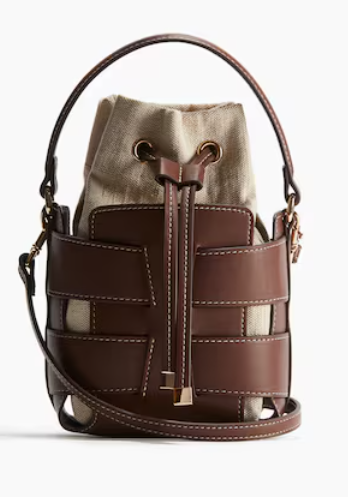
\includegraphics[width=0.65\textwidth]{ f95ece428f1f455cbac29e0cd7748163.png }\hfill\null

\vspace*{0.5ex}

% ---- Résumé -----------------------------------------------------------------
\headleft{Profile Summary}
Data Scientist with 4+ years of experience turning complex data into business-driven insights and AI solutions. Strong background in statistics, machine learning and data engineering with proven ability to deliver predictive models, dashboards and NLP applications in production. Passionate about leveraging data to optimise decision-making and create value.

% ---- Contact ----------------------------------------------------------------
\headleft{Contact details}\small
\MVAt\ {\small papesalioufall2@gmail.com} \\[0.4ex]
\Mobilefone\ 0753481453 \\[0.5ex]
\Letter\ 38 Rue de Paris, 75010 Paris, France
\normalsize

% ---- Infos perso ------------------------------------------------------------
\headleft{Personal information}
Citizenship: \textbf{Sénégalaise} \\[0.5ex]
Family: \textbf{Célibataire} \\[0.5ex]
Languages: \textbf{Français (natif), Anglais (courant)}

% ---- Compétences ------------------------------------------------------------
\headleft{Skills}
\begin{itemize}
  \item Python
  \item R
  \item SQL
  \item PySpark
  \item Machine Learning
  \item Deep Learning
  \item NLP
  \item TensorFlow \& Keras
  \item Scikit-learn
  \item Docker \& Git
  \item Airflow
  \item Power BI \& Tableau
  \item Data Visualization
  \item Statistics
  \item Cloud (AWS, GCP)
\end{itemize}

\end{minipage}\kern 0.09\textwidth
}
\end{minipage}
% ============================================================================
%                               COLONNE DROITE
% ============================================================================
\hskip2.5em
\begin{minipage}[t]{0.56\textwidth}
\setlength{\parskip}{0.8ex}
\vspace{2ex}

% ------------------------ EXPÉRIENCE ----------------------------------------
\headright{Experience}
\textsc{Data Scientist} at \textit{AXA France} (Paris, France)  \dates{Mar 2022–Present} \\
\smaller{Développé des modèles de scoring risque crédit (AUC +8~\%).}\is
\smaller{Implémenté un pipeline MLOps (Docker, Airflow, GitLab CI/CD) réduisant de 40~\% le temps de mise en production.}\is
\smaller{Mis en place un tableau de bord Power BI permettant aux équipes métiers de suivre en temps réel les KPIs sinistralité.}\is
\smaller{Collaboré avec les équipes actuariat et IT pour automatiser la collecte de données (Spark, AWS S3), diminuant de 25~\% le temps de traitement mensuel.}\is

\textsc{Data Analyst} at \textit{Orange} (Dakar, Senegal)  \dates{Sep 2019–Feb 2022} \\
\smaller{Analyse des données de réseau mobile pour identifier les zones de congestion ; recommandations ayant amélioré la QoS de 15~\%.}\is
\smaller{Création de modèles de prévision de churn (Random Forest, XGBoost) avec une précision de 82~\%.}\is
\smaller{Construction de dashboards Tableau consultés par +50 utilisateurs métiers pour le suivi quotidien des indicateurs de vente.}\is
\smaller{Formation de 10 collègues aux bonnes pratiques SQL et visualisation de données.}\is

% ------------------------ ÉDUCATION ----------------------------------------
\headright{Education}
\textsc{Master of Science – Data Science}. \textit{Université Paris-Saclay}. \dates{2017–2019} \\
\textsc{Licence – Mathématiques appliquées et Informatique}. \textit{Université Cheikh Anta Diop de Dakar}. \dates{2014–2017} \\

% ------------------------ CERTIFICATIONS ------------------------------------
\headright{Certifications}
\smaller{\textsc{TensorFlow Developer Certificate}}, \textit{Google / DeepLearning.AI}. \dates{Jun-2023} \\
\smaller{\textsc{IBM Data Science Professional Certificate}}, \textit{Coursera \& IBM}. \dates{Dec-2021} \\

% ------------------------ HOBBIES -------------------------------------------
\headright{Hobbies}
\textit{Football, échecs, photographie, voyages}

\end{minipage}

\end{document}